% \iffalse meta-comment
%
% Copyright (C) 2025 Cynthia Rodriguez
% --------------------------------
%
% This file may be distributed and/or modified under the
% conditions of the LaTeX Project Public License, either version 1.3
% of this license or (at your option) any later version.
% The latest version of this license is in:
%
% http://www.latex-project.org/lppl.txt
%
% and version 1.3c or later is part of all distributions of LaTeX
% version 2008-05-04 or later.
%
% \fi
%
% \iffalse
%<*driver>

\ProvidesFile{pubQuiz.dtx}
%</driver>
%<class>\NeedsTeXFormat{LaTeX2e}[2023-11-01]
%<class>\ProvidesClass{pubQuiz}
%<*class>[2025-06-29 v1.0.1 A class for generating Pub Quiz scripts and answer sheets]
%</class>


%<*batchfile>
\begingroup
\input docstrip.tex
\keepsilent
\askforoverwritefalse
\usedir{tex/latex/pubQuiz}
\generate{\file{pubQuiz.cls}{\from{pubQuiz.dtx}{class}}}
\obeyspaces
\endgroup
%</batchfile>

%<*driver>
\documentclass{ltxdoc}
\EnableCrossrefs
\CodelineIndex
\RecordChanges

\RequirePackage{multicol}
\RequirePackage{graphicx}
\RequirePackage{listings}
\RequirePackage{tikz}
\RequirePackage[export]{adjustbox}
\RequirePackage[columns=2]{idxlayout}

\begin{document}
	\DocInput{pubQuiz.dtx}
\end{document}
%</driver>
%\fi

% \changes{v1.0}{2025-06-27}{Initial version}
%
% \GetFileInfo{pubQuiz.dtx}
% \def\filename{pubQuiz}
% \def\fileversion{v1.0.2}
% \def\filedate{2025-07-14}
%
%	\DoNotIndex{\DeclareOption,\RequirePackage,\PassOptionsToClass,\CurrentOption,\ProcessOptions,\relax,\LoadClass,\maketitle,\par,\PubInstructions,\vspace}
%	\DoNotIndex{\newif,\else,\fi,\begin,\end,\foreach,\includegraphics,\item,\let,\makeatletter,\makeatother,\NewDocumentEnvironment,}
%	\DoNotIndex{\NewEnviron,\DeclareOption,\NewDocumentCommand,\IfNoValueTF,\IfNoValueT,\IfNoValueF,\IfBlankTF,\IfBlankT,\IfBlankF,\IfBooleanF,\IfBooleanTF,\IfBooleanT}
%	\DoNotIndex{\titleformat,\titlespacing,\section,\subsection,\subsubsection,\thesection,\thesubsection,\thesubsubsection}
%	\DoNotIndex{\huge,\Large,\large,\filcenter,\textbf,\texttt,\textit,\textsc,\underline}
%	\DoNotIndex{\setlength,\setlist,\abovedisplayskip,\pagestyle,\clearpage,\noindent,\enspace,\hrulefill,\hfill,\phantom,\nicefrac}
%	\DoNotIndex{\multicolsep,\columnsep,\columnwidth,\columnwidth}
%	 \DoNotIndex{\ifpubQuiz@Host,\pubQuiz@Hosttrue,\pubQuiz@Hostfalse}
%	\DoNotIndex{\ifpubQuiz@Answers,\pubQuiz@Answerstrue,\pubQuiz@Answersfalse}
%	 \DoNotIndex{\ifpubQuiz@Bonus,\pubQuiz@Bonustrue,\pubQuiz@Bonusfalse}
%	\DoNotIndex{\ifpubQuiz@Columns,\pubQuiz@Columnstrue,\pubQuiz@Columnsfalse}
% 	\DoNotIndex{\begingroup,\endgroup,\newcommand,\LoadClass,\LaTeX,\\,\dotfill,\endPubInstructions,\endpubQuizHide,\endPubRules,\fill,\hspace,\i}

% \title{The \textsf{\filename} class
% \thanks{This document corresponds to \textsf{\filename}~\fileversion, dated \filedate.}}
% \author{Cynthia Rodriguez \\ \texttt{CR.github@pm.me}}
% \date{Version \fileversion, \filedate}
%
% \maketitle
%
% 	\begin{abstract}
%		This manual describes how to use the pubQuiz class to generate sheets for running a Pub Quiz or Trivia
%			activity. 
%		The package creates simple answer sheets for the participants, and gives the option
%			to generate a script for the host of the event.
% 	\end{abstract}
%
%	\tableofcontents
%	\clearpage
%
% 	\section{Examples}
%		 \lstset{
%			language=TeX,
%			keywords=[4]{begin,PubRound,PubCat,end,documentclass},
%			keywordstyle=\color{black!50!green},
%			commentstyle=\color{black!60},
%			tabsize=2,
%			frame=single
%		}
% 		\subsection{An unscripted example}
%			Quizzard, the renowned Pub Quiz master, has agreed to make the answer sheets for this week's Quiz at the \LaTeX pub.
%			A new assistant will be designing the questions this week, so it should be an easy task.
%
%			The quiz will have only one round with five standard categories and a bonus game:
%			\begin{enumerate}
%				\item Beer: 5 questions
%				\item Spirits: 5 questions
%				\item Sports: 5 questions
%				\item BONUS: Darts Game
%				\item Wines: 5 questions
%				\item Name the Song: 20 questions
%			\end{enumerate}
%			Quizzard wants the Name the Song category to show the answers in 4 columns.
%
%			Luckily, Quizzard has been using \LaTeX for a long time, and he has just discovered the \texttt{PubQuiz} class, which seems well-suited for the task.
%			The main commands for making answer sheets are:		\changes{v1.0.1}{2025-06-29}{Edited for clarity}
%			\begin{itemize}
%				\item \texttt{$\backslash$PubRound}: prints the Team Name space, the Score box (optional: with the points available), and the Round title
%				\item \texttt{$\backslash$PubCat}: prints the answer lines for a category. By default, it prints 5 answer lines in a single column,
%					but it allows for Bonus categories, multiple columns, and other numbers of questions.
%			\end{itemize}
%			 \changes{v1.0.1}{2025-06-29}{Added bonus category clarification}
%			In Bonus categories, the answer sheet will have the category title with no answer lines.
%
%			With this information, Quizzard creates their first \texttt{pubQuiz} document:
%			\lstinputlisting{./Examples/unscriptedQuizzard.tex}
%			Quizzard looks at the compiled answer sheet, and is happy with the outcome:
%			\begin{center}
%				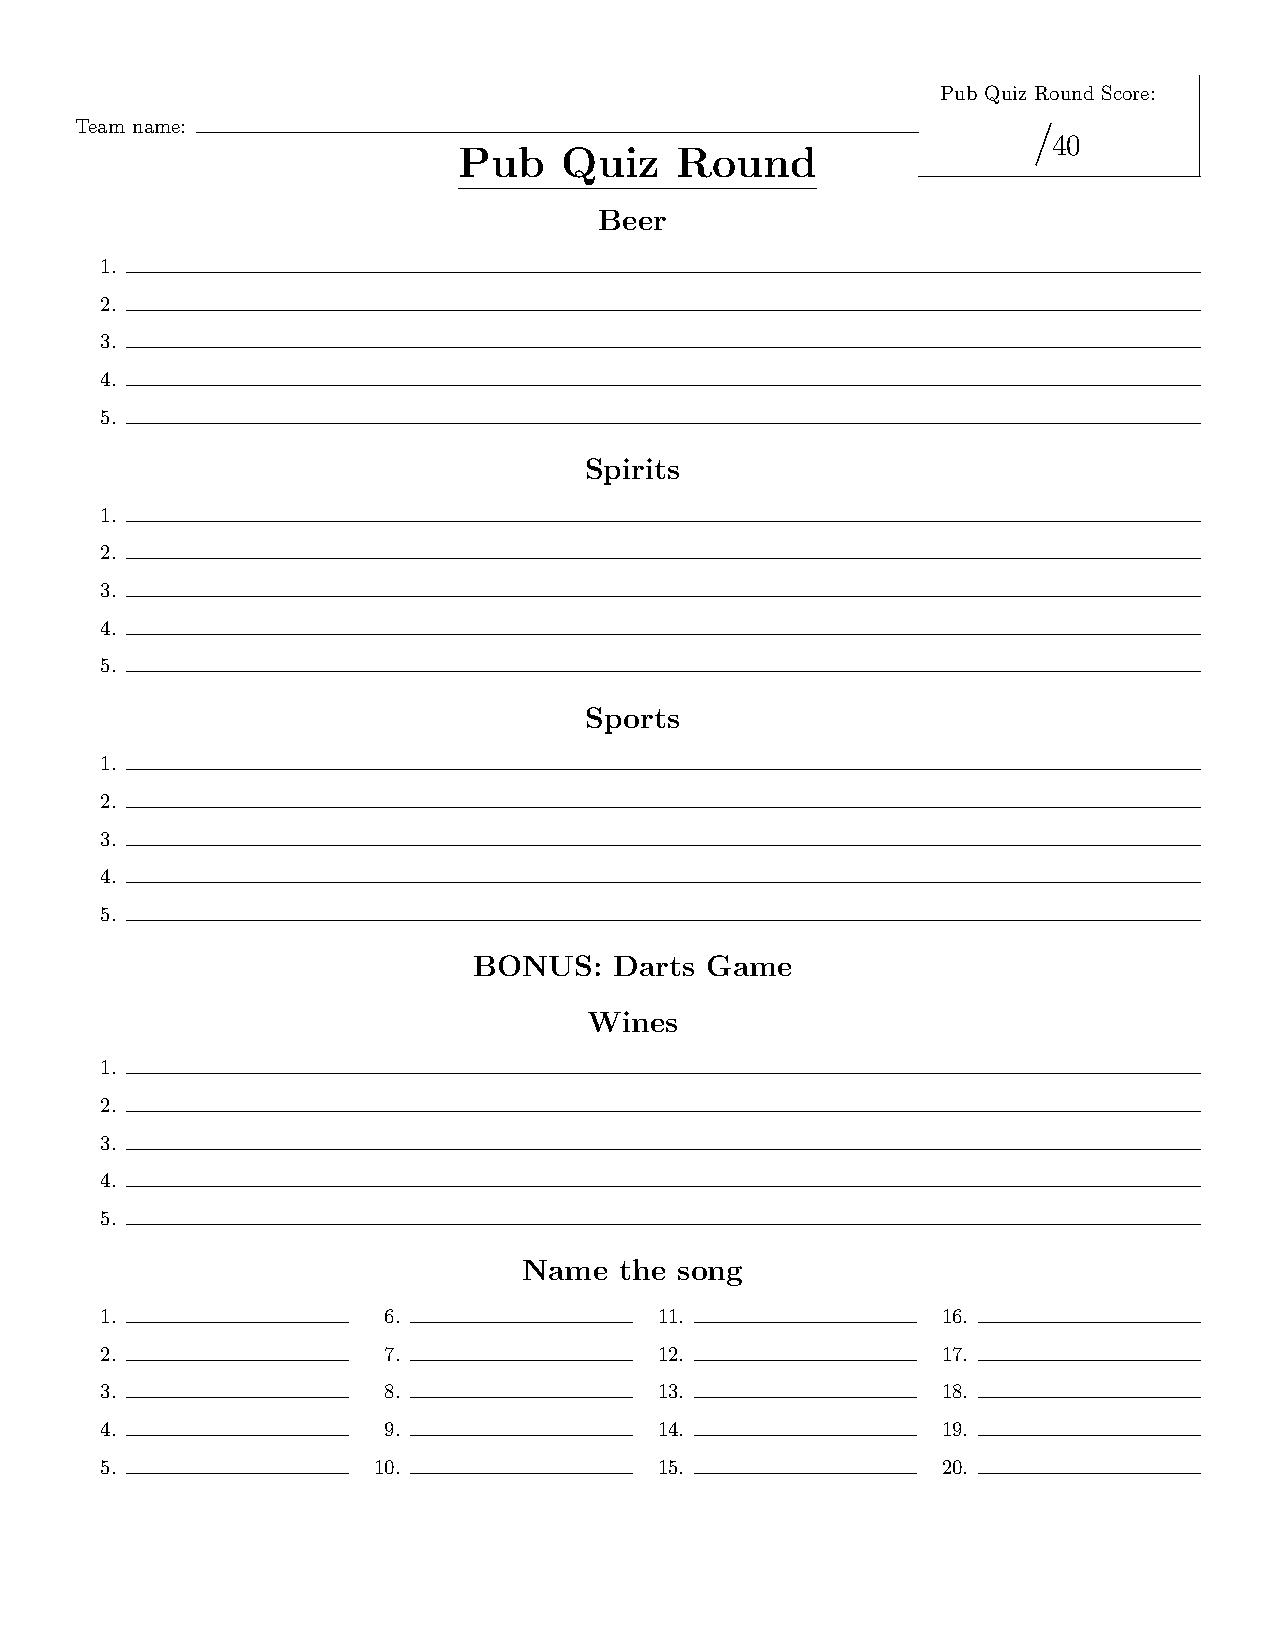
\includegraphics[width=\textwidth,frame]{./Examples/unscriptedQuizzard}
%			\end{center}
%
%		\clearpage
%		\subsection{A scripted example}
%			Quizzard's assistant has taken a vacation, so Quizzard will have to plan this week's Pub Quiz alone.
%			That means writing a script with questions and answers, as well as the answer sheets. 
%			He decides to plan a short trivia, with two categories and a bonus game:
%			\begin{enumerate}
%				\item Ducks: 5 questions
%				\item BONUS: Coin Toss
%				\item Duck songs: 10 questions
%			\end{enumerate}
%			Quizzard looks again at the \texttt{PubQuiz} class, which he hopes will help him in this task.
%			The main commands/environments to use for scripts and answer sheets  are:
%			\begin{itemize}
%				\item To print a script, one should give the \texttt{host} option to the \texttt{pubQuiz} class.
%				\item The environment \texttt{PubRules} allows for the Pub Quiz rules to be written in the host script.
%				\item The environment \texttt{PubInstructions} allows for instructions for the hosts to be written in the host script.
%				\item \texttt{$\backslash$PubRound}: prints the Team Name space, the Score box (optional: with the points available), and the Round title.
%				\item Environment \texttt{PubCategory}: prints the category title (with some extra details), questions given as in an \texttt{enumerate} environment.
%						The environment allows for Bonus categories, multiple columns, category instructions, and some host notes.
%				\item \texttt{$\backslash$PubQ}: for giving a question and its answer. A dot between question and answer prints them inline in the host script.
%			\end{itemize}
%			As before, Bonus categories in the answer sheet will have the category title with no answer lines.
%			
%			With this information, Quizzard creates their first \texttt{pubQuiz} scripted sheet:
%				\lstinputlisting{./Examples/scriptedQuizzard.tex}
%			Quizzard looks at the compiled output and gets this answer sheet
%			\begin{center}
%				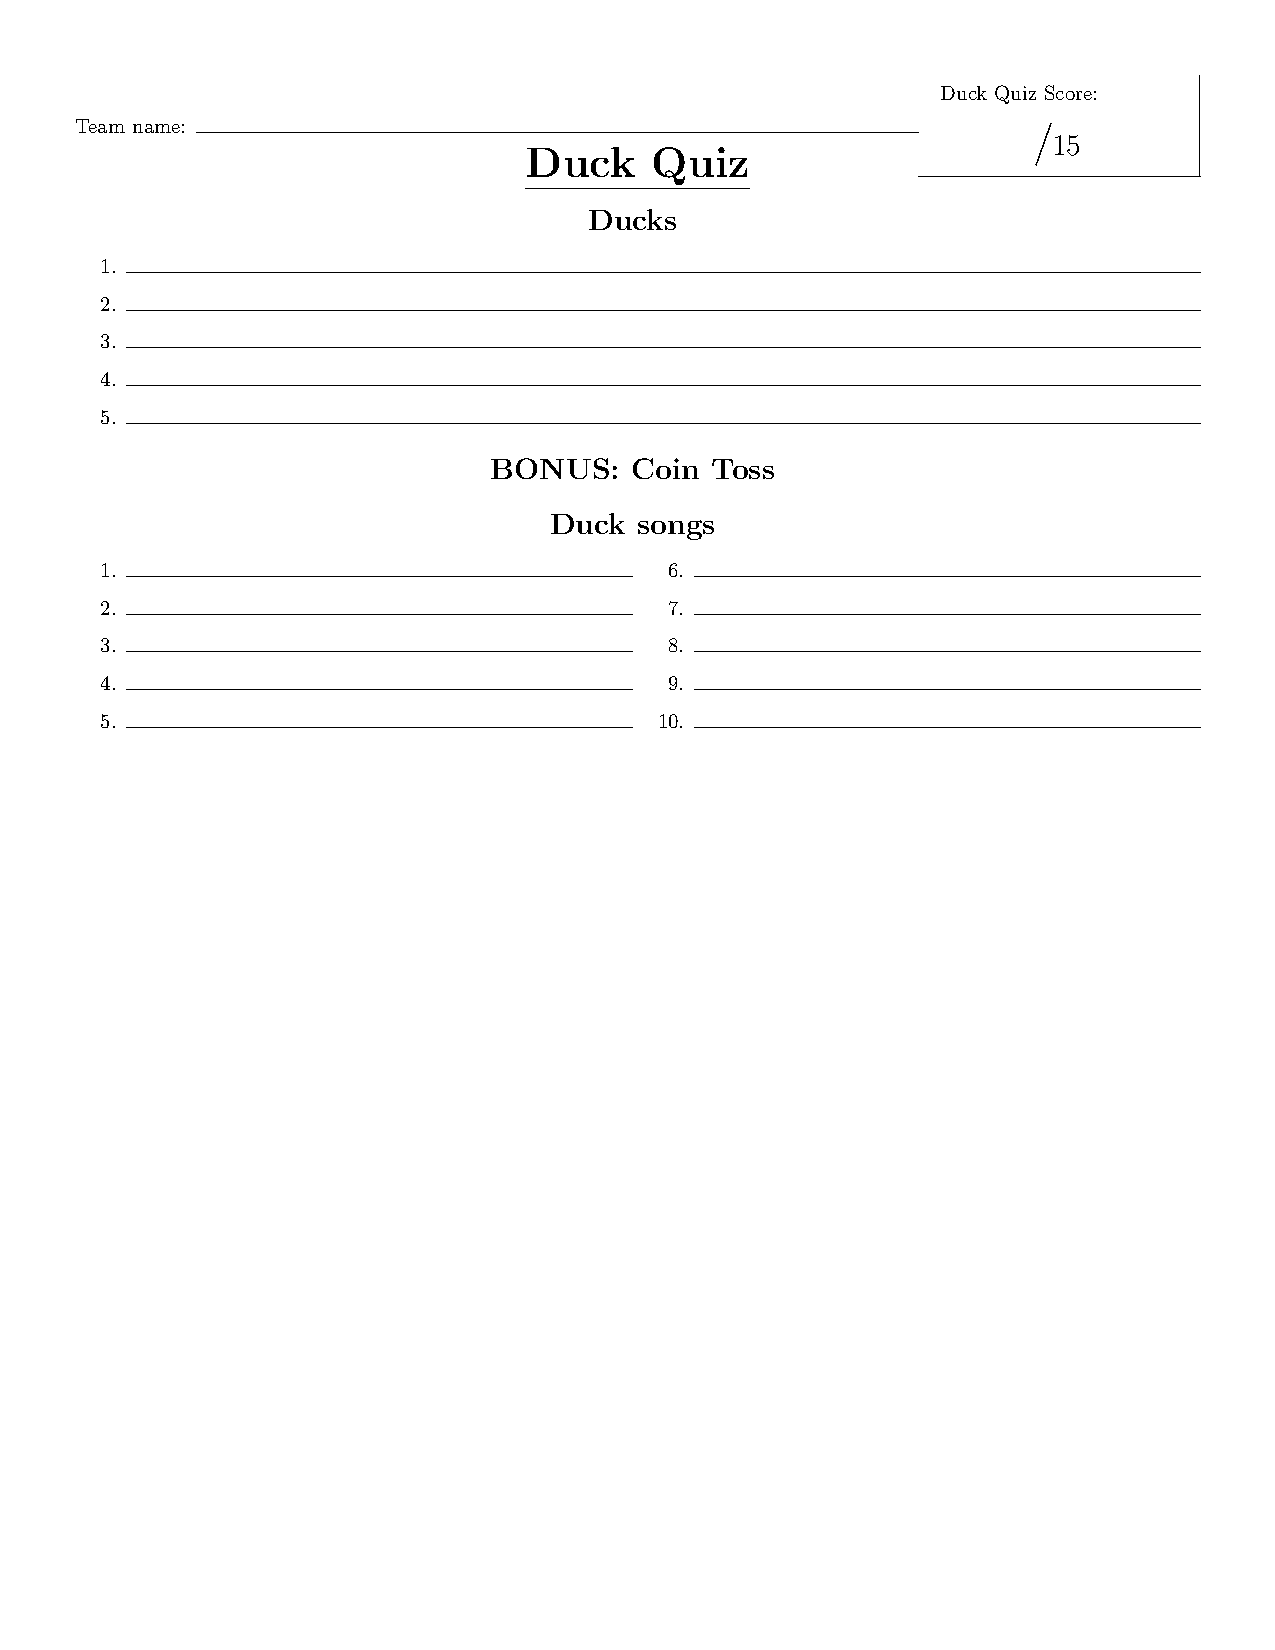
\includegraphics[width=\textwidth,frame]{./Examples/scriptedQuizzard}
%			\end{center}
%			To produce the host script, Quizzard gives the \texttt{host} option to the class.
%				\lstinputlisting{./Examples/scriptedQuizzardHost.tex}
%			The compiled output then becomes a host script
%			\begin{center}
%				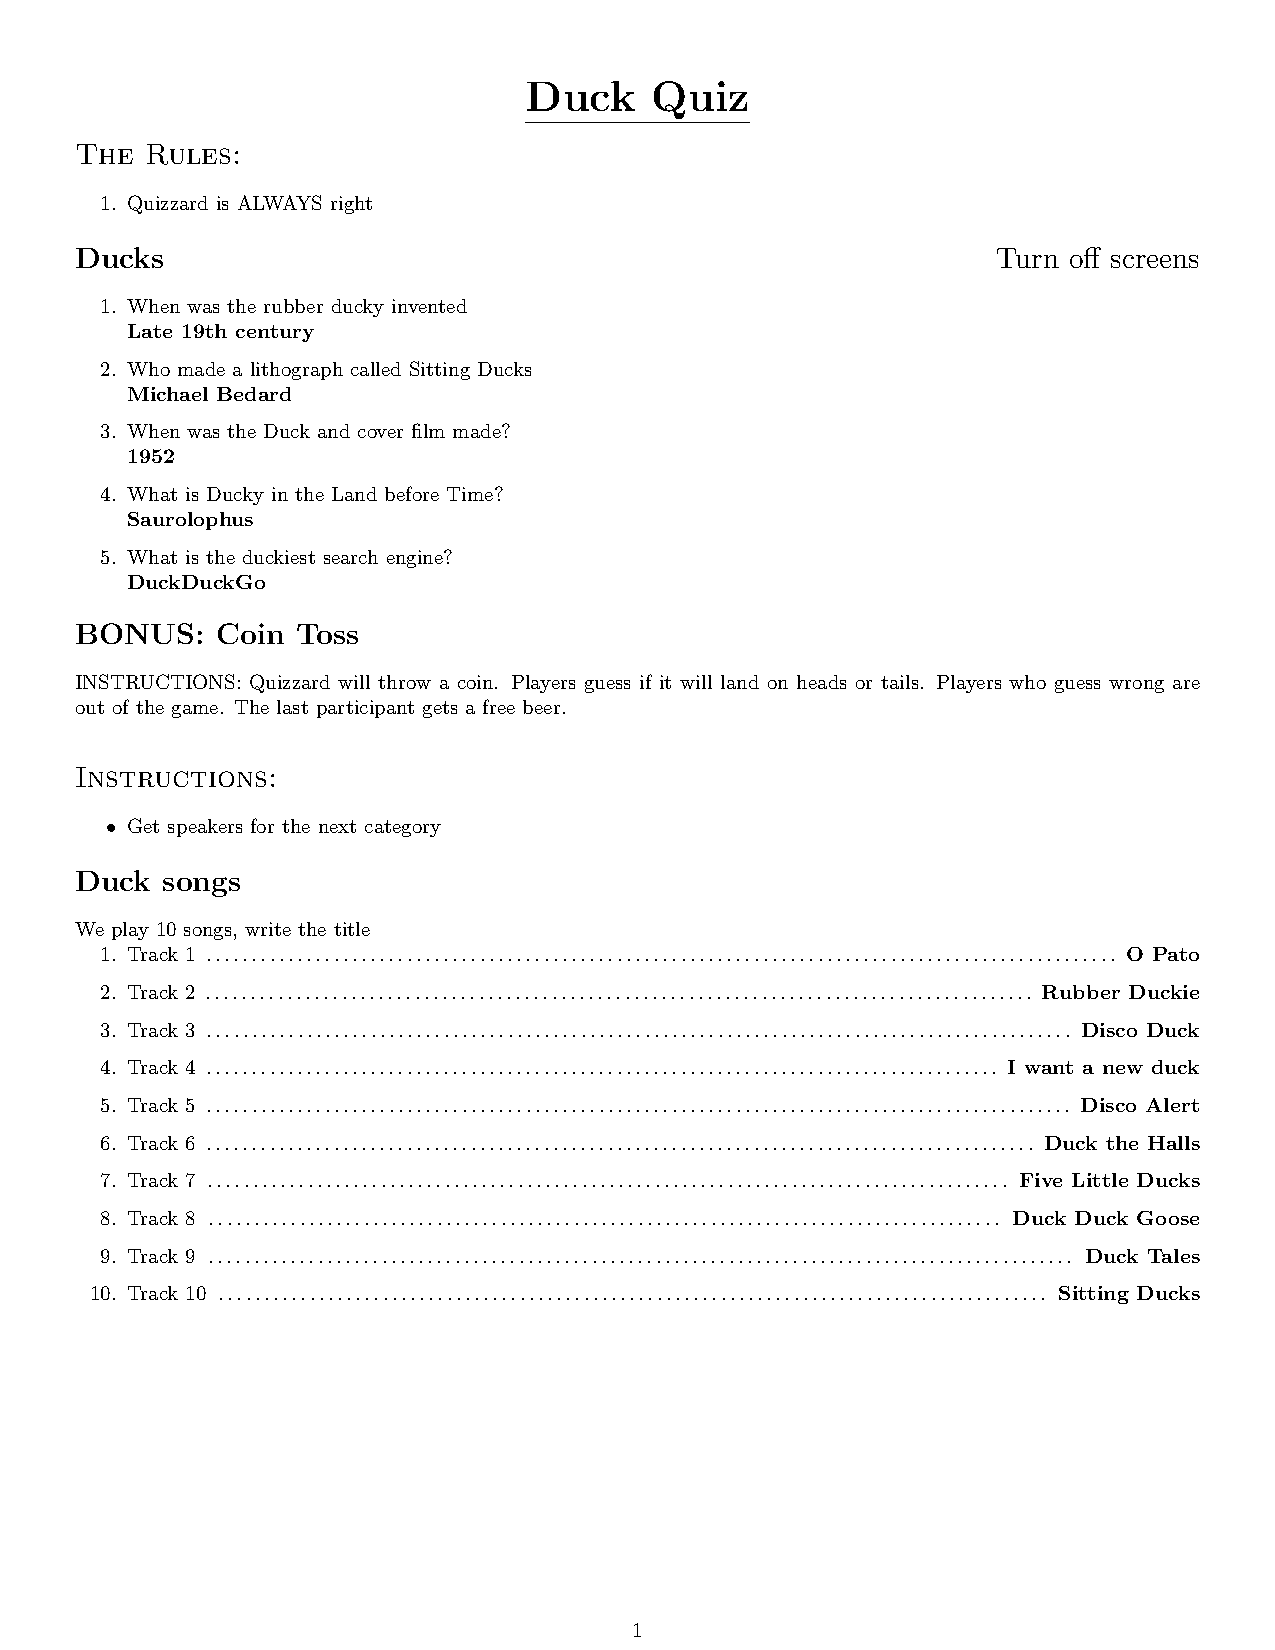
\includegraphics[width=\textwidth,frame]{./Examples/scriptedQuizzardHost}
%			\end{center}
%		\clearpage
%		\subsection{A picture page}
%			As part of the Duck Quiz, Quizzard would like to have a name the duck picture page.
%			The only extra command is 
%			\begin{itemize}
%				\item \texttt{$\backslash$PubQPic}: for giving a picture question and its answer.
%			\end{itemize}
%			With this information, Quizzard creates their first \texttt{pubQuiz} picture page:
%				\lstinputlisting{./Examples/pictureQuizzard.tex}
%			Quizzard looks at the compiled output and gets this answer sheet
%			\begin{center}
%				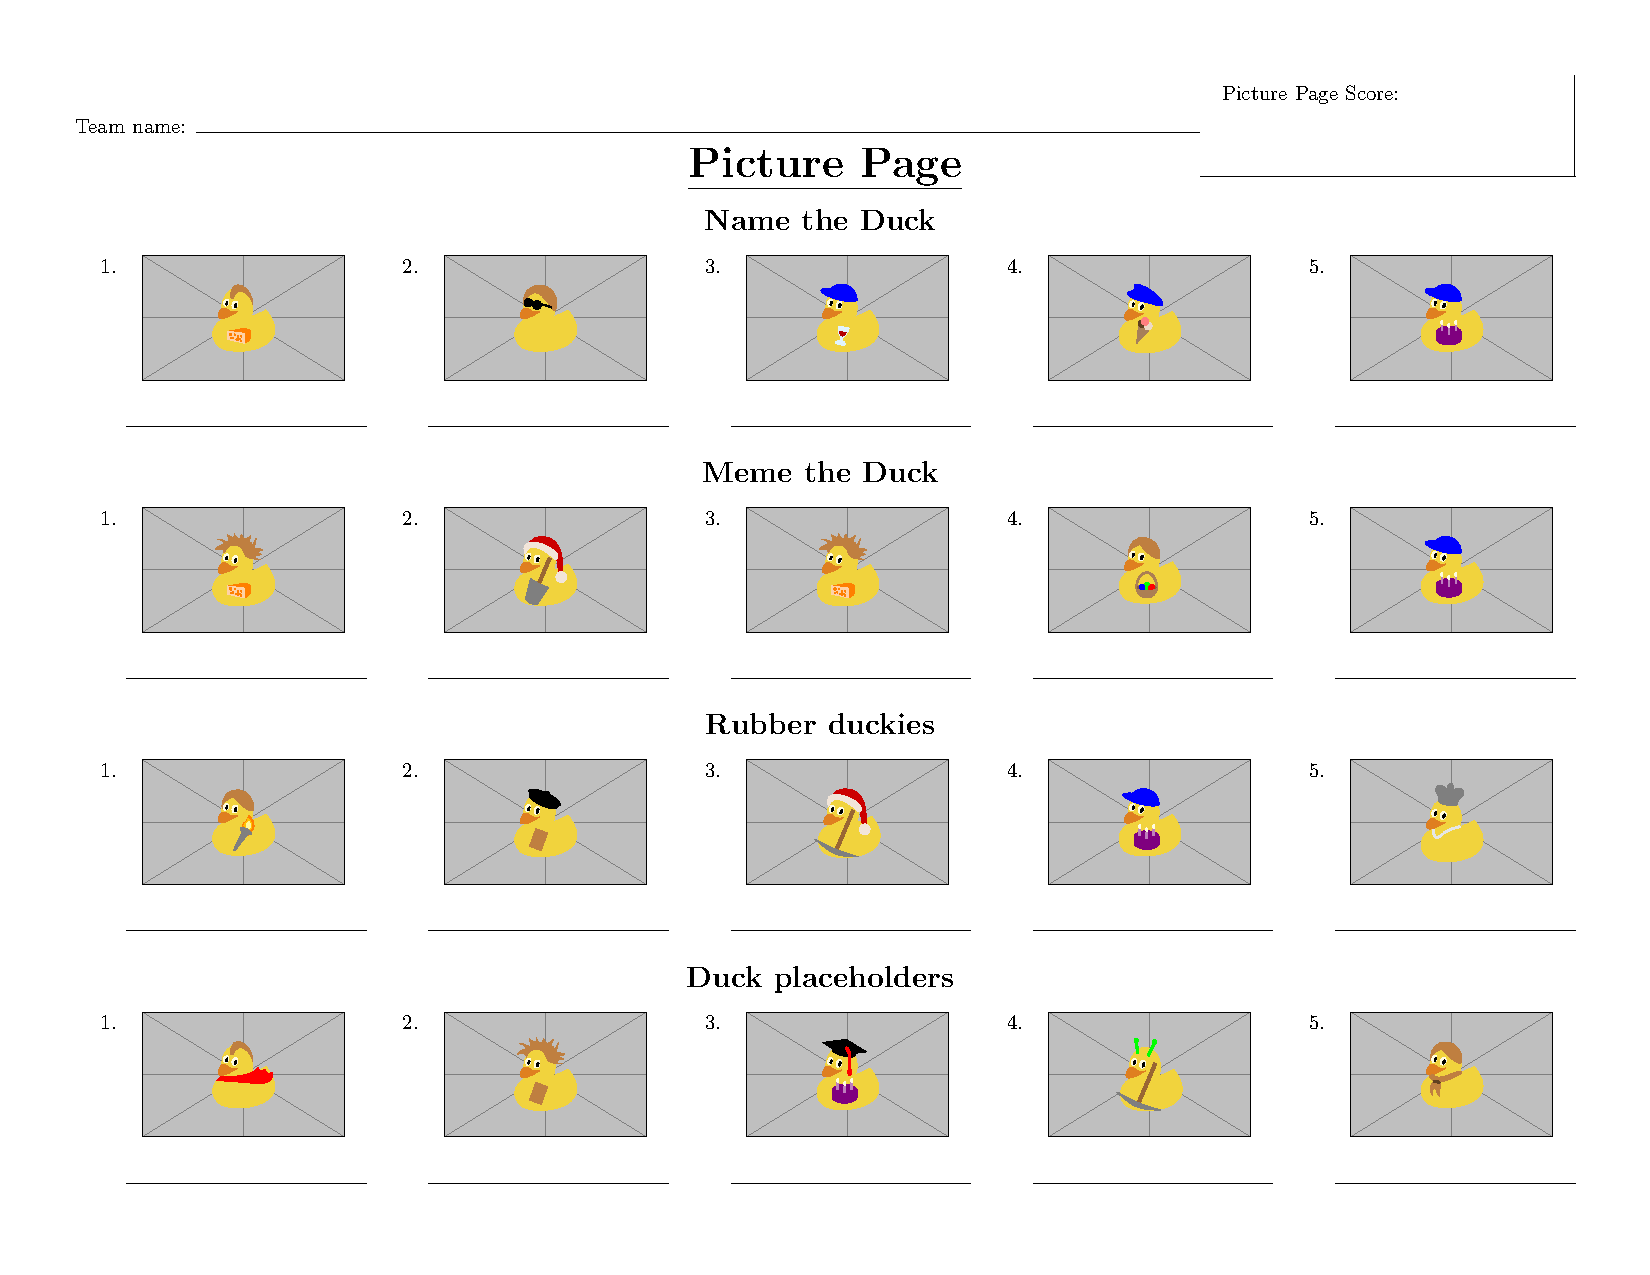
\includegraphics[width=\textwidth,frame]{./Examples/pictureQuizzard}
%			\end{center}
%			To produce the host script, Quizzard gives the \texttt{host} option to the class.
%				\lstinputlisting{./Examples/pictureQuizzardHost.tex}
%			The compiled output then becomes a host script
%			\begin{center}
%				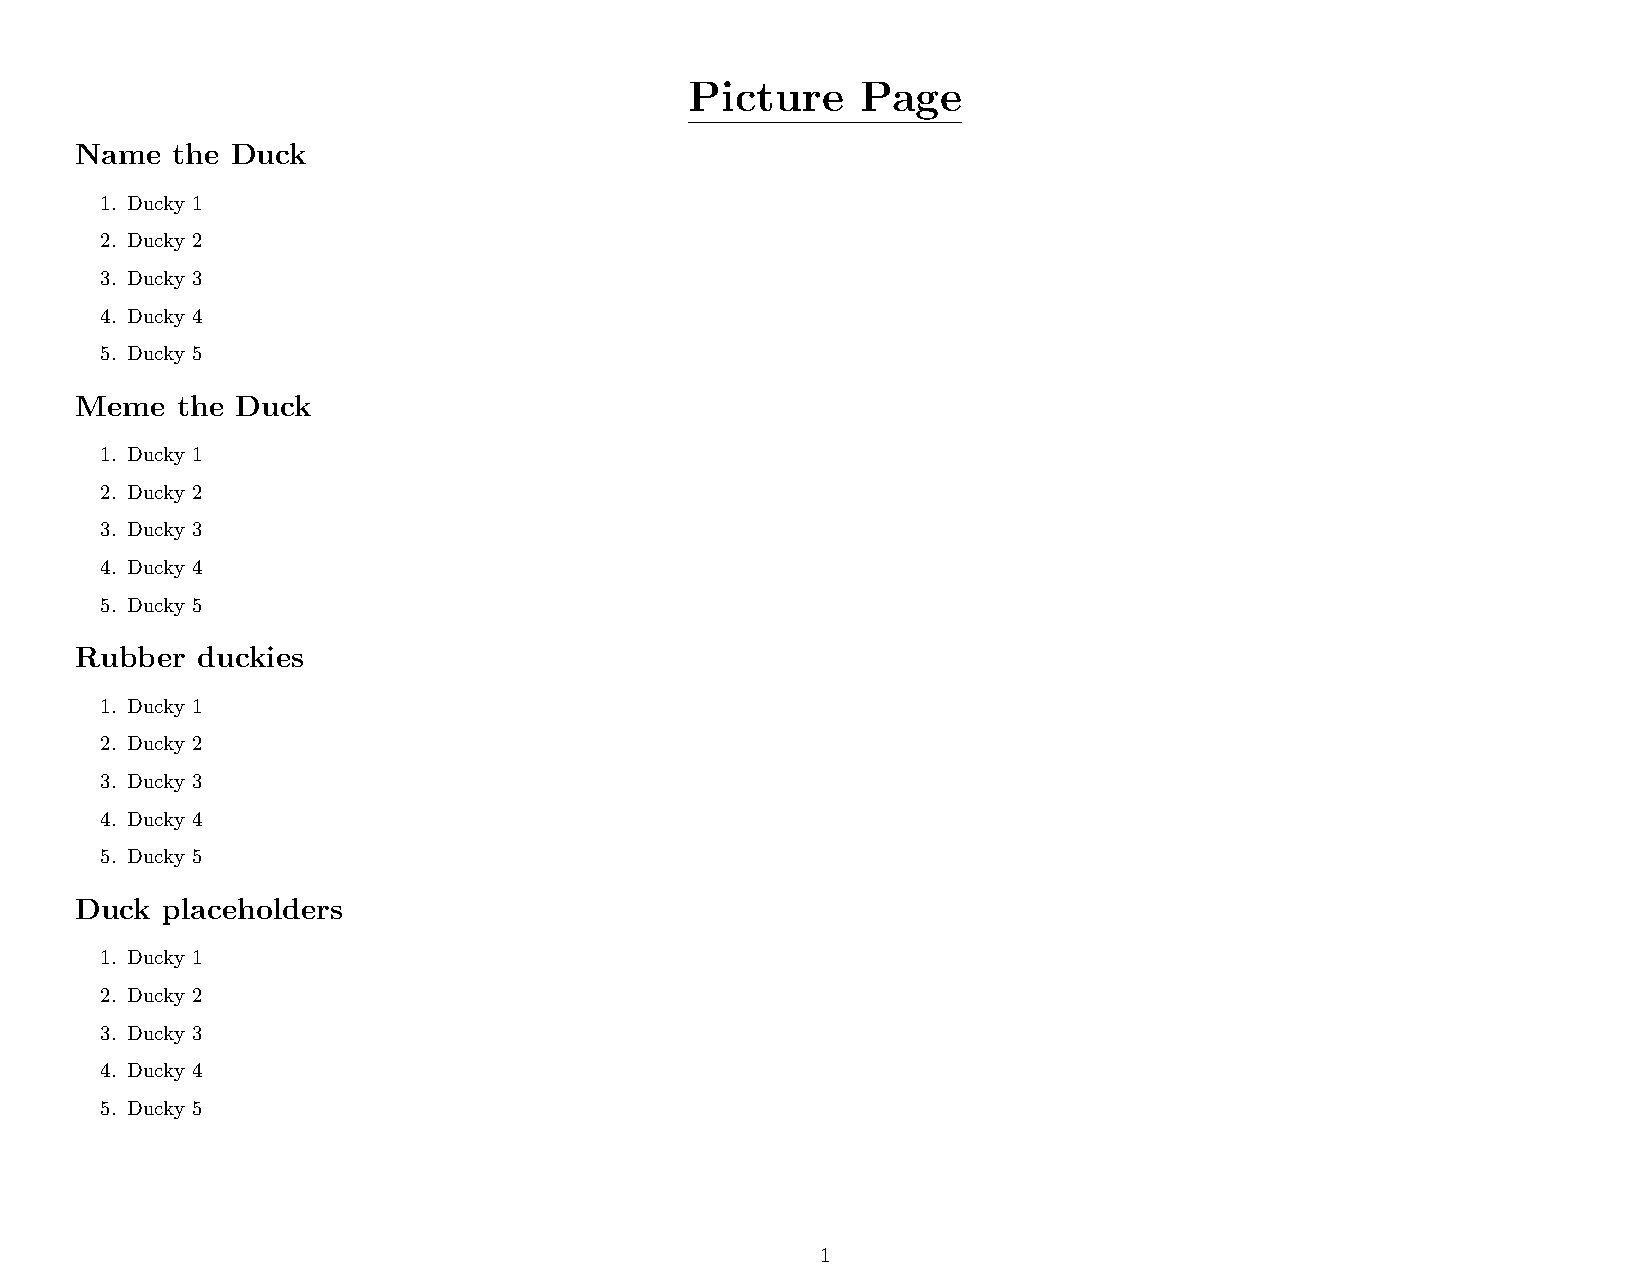
\includegraphics[width=0.95\textwidth,frame]{./Examples/pictureQuizzardHost}
%			\end{center}
%			
%
% 	\section{User Commands}
%		The PubQuiz class can create both answer sheets and host scripts for a Pub Quiz style event. 
%		We have made the choice to keep the number of user commands small, and enable functionality via
%			tokens and optional parameters, which we will explain here.

%		\subsection{Class Options}
%			\NewDocElement{ClassOption}{option}
%			The class inherits all options from the \texttt{article} class, and adds three extra options for easier 
%				PubQuiz creation:
%			\begin{itemize}
%				\item \texttt{host} and \texttt{nohost}: 
%					\begin{itemize}
%						\item \DescribeClassOption{host}  
%							The \texttt{host} option creates a document for the hosts.\\
%							It creates a script with rules, instructions, questions to read (with or without answers) for 
%							regular and bonus categories. 
%						\item \DescribeClassOption{nohost} 
%							The \texttt{nohost} option is enabled by default and creates a document for participants.\\
%							It creates an answer sheet with space to write team names, a score box, category titles
%							and space for answers, and titles for bonus categories (if this is enabled).
%							Answer spaces are not given for bonus categories.
%					\end{itemize}
%				\item \texttt{answers} and \texttt{noanswers}: 
%					\begin{itemize}
%						\item \DescribeClassOption{answers}  
%							The \texttt{answers} option is enabled by default and affects only the document for hosts.\\
%							It prints the given answers to all questions in the host script.
%						\item \DescribeClassOption{noanswers}  
%							The \texttt{noanswers} option disables including correct answers in the host document.
%					\end{itemize}
%				\item \texttt{printbonus} and \texttt{noprintbonus}: 
%					\begin{itemize}
%						\item \DescribeClassOption{printbonus}  
%							The \texttt{printbonus} option is enabled by default and affects only the 
%							document for participants.\\
%							When it is enabled, the title of bonus categories is printed in the answer sheet.
%						\item \DescribeClassOption{noprintbonus}  
%						When the \texttt{noprintbonus} option is chosen, bonus categories do not appear 
%							in the answer sheets for participants.
%					\end{itemize}
%			\end{itemize}

%		\subsection{Setting up a Pub Quiz}
% 			\DescribeMacro{\PubRound}
%			The basic set-up command for a Pub Quiz document is 
%				\begin{center}
%					$\backslash$PubRound\{round\_name\}[max\_points]
%				\end{center}
%				which takes two parameters
%				\begin{itemize}
%					\item \texttt{round\_name}: Name to be printed for the round (mandatory)
%					\item \texttt{max\_points}: Maximum points in the round (optional)
%				\end{itemize}
%				This command behaves differently in the host script and the answer sheet.
%				\begin{itemize}
%					\item Host script: Prints only the round title
%					\item Answer sheet: Prints three things on the page:
%						\begin{enumerate}
%							\item Line for participants to write their team name
%							\item Score box (maximum score included, if given)
%							\item Round title
%						\end{enumerate}
%				\end{itemize}
%
%			The class also provides two  environments for hosts to add instructions in the host script:
%			\begin{itemize}
%				\item \DescribeEnv{PubRules} 
%					The environment \texttt{PubRules} which creates the document title, 
%						prints the headline \textsc{The Rules.} and opens a numbered list. 
%					The user writes their rules as in an \texttt{enumerate} environment.
%				\item \DescribeEnv{PubInstructions} 
%					The environment \texttt{PubInstructions} prints the headline \texttt{Instructions:} and 
%						opens a non-numbered list. 
%					The user writes their instructions as in an \texttt{itemize} environment.
%			\end{itemize}	
	
%		\subsection{Creating Categories}
%			The \texttt{PubQuiz} class includes three commands to create categories and subcategories 
%				in a Pub Quiz document.

%			\DescribeMacro{\PubCat} The first one is \texttt{$\backslash$PubCat}, which allows the quick creation 
%				of answer sheets, without a host script.
%				\begin{center}
%					$\backslash$PubCat * $\vert$number\_columns$\vert$ \{category\_name\} [num\_questions]
%				\end{center}
%				\begin{itemize}
%					\item The star is an optional argument which signals a bonus category.
%						If it is given, no spaces to answer will be printed in the answer sheet.
%					\item The optional parameter \texttt{number\_columns} allows printing the answer lines in 
%						several columns within an answer sheet. 
%						The minimum value for \texttt{number\_columns} is $2$.
%					\item The only mandatory parameter is \texttt{category\_name}, which determines the name
%						to be printed for the category. 
%					\item The optional parameter \texttt{num\_questions} gives the number of questions in the category.
%						This value is set to be 5 by default.
%				\end{itemize}
%
%			\DescribeEnv{PubCategory}
%			For scripted pubQuiz documents, the corresponding environment is \texttt{PubCategory}.
%			 \changes{v1.0.1}{2025-06-29}{Added PubCategory environment with ordered parameters}
%				\begin{center}
%					$\backslash$begin\{\texttt{PubCategory}\} * $\vert$\texttt{number\_columns}$\vert$ \{\texttt{category\_name}\} $<$\texttt{host\_notes}$>$
%						[\texttt{host\_instructions}] \\
%						\ldots \\
%					$\backslash$end\{\texttt{PubCategory}\}
%				\end{center}
%			The environment accepts the following parameters:
%				\begin{itemize}
%					\item The star is an optional argument which signals a bonus category.
%						If it is given, no spaces to answer will be printed in the answer sheet.
%					\item The optional parameter \texttt{number\_columns} allows printing the answer lines in 
%						several columns within an answer sheet. 
%						The minimum value for \texttt{number\_columns} is $2$.
%					\item The only mandatory parameter is \texttt{category\_name}, which determines the name
%						to be printed for the category. 
%					\item The optional parameter \texttt{host\_notes} allows for short notes on the host script.
%						The notes are printed inline with the category name, using the same format.
%					\item The optional parameter \texttt{host\_instructions} allows for longer category instructions on the host script.
%						The notes are printed before the questions in the category, using the standard text format.
%				\end{itemize}
%			
%			\DescribeEnv{PubSubcategory}
%			Scripted \texttt{pubQuiz} documents also allow for the inclusion of subcategories with the 
%				command \texttt{$\backslash$PubSubcategory}.
%			 \changes{v1.0.1}{2025-06-29}{Added PubSubcategory environment with ordered parameters}
%				\begin{center}
%					$\backslash$begin\{\texttt{PubSubcategory}\} * $\vert$\texttt{number\_columns}$\vert$ \{\texttt{category\_name}\} $<$\texttt{host\_notes}$>$
%						[\texttt{host\_instructions}] \\
%						\ldots \\
%					$\backslash$end\{\texttt{PubSubcategory}\}
%				\end{center}
%			The environment accepts the following parameters:
%				\begin{itemize}
%					\item The star is an optional argument which signals a bonus category.
%						If it is given, no spaces to answer will be printed in the answer sheet.
%					\item The optional parameter \texttt{number\_columns} allows printing the answer lines in 
%						several columns within an answer sheet. 
%						The minimum value for \texttt{number\_columns} is $2$.
%					\item The only mandatory parameter is \texttt{subcategory\_name}, which determines the name
%						to be printed for the category. 
%					\item The optional parameter \texttt{host\_notes} allows for short notes on the host script.
%						The notes are printed inline with the subcategory name, using the same format.
%					\item The optional parameter \texttt{host\_instructions} allows for longer category instructions on the host script.
%						The notes are printed before the questions in the subcategory, using the standard text format.
%				\end{itemize}
%			 \changes{v1.0.1}{2025-06-29}{Added clarification on the difference between  \texttt{$\backslash$PubCategory} and  \texttt{$\backslash$PubSubcategory}}
%			Note that the parameters of \texttt{$\backslash$PubSubcategory} are identical to those of 
%				\texttt{PubCategory}. However, \texttt{$\backslash$PubSubcategory} must be nested within a \texttt{$\backslash$PubCategory} environment.
%
%
%		\subsection{Creating Questions}
%			The \texttt{PubQuiz} class gives two commands to include questions (and their answers) in the script.
%
%			The command \texttt{$\backslash$PubQ} is used to write text-based questions.
%			In the host script, it prints the question and its answer (if the \texttt{printanswers} option is enabled).
%			In the answer sheet, it prints the question number and a line for participants to write their answer on (for non-bonus questions)
%				\begin{center}
%					$\backslash$PubQ * \{question\} . [answer]
%				\end{center}
%				\begin{itemize}
%					\item A star is an optional argument which signals a bonus question.
%						If it is given, nothing will be printed in the answer sheet.
%					\item The text for the question is given as the optional parameter \texttt{question}.
%						If no text is given, ``No question given'' will be printed in the host script.
%					\item A dot is an optional argument which indicates that the answer should be written inline with the question, with dots separating them.
%						If it is not given, the answer will be printed in a new line.
%					\item The answer for the question is given as the optional parameter \texttt{answer}.
%				\end{itemize}
 
%				For picture-based questions, the command \texttt{$\backslash$PubQPic} is given.
%				In the answer sheet, it prints the question number, an image and a line below it for participants to write their answer.
%				In the host script, only the question number and the answer are printed.
%				\begin{center}
%					$\backslash$PubQPic  \{image\_file\}[answer]
%				\end{center}
%				\begin{itemize}
%					\item The path to the image file should be given as the mandatory parameter \texttt{image\_file}
%					\item The answer for the question is given as the optional parameter \texttt{answer}.
%				\end{itemize}
%
%
% \MaybeStop{\PrintIndex}
%
%
%\section{Implementation}
%	List of required packages for options:
%    \begin{macrocode}
	\RequirePackage{ifthen}
	\RequirePackage{environ}
%    \end{macrocode}
%	Switch \DescribeClassOption{host} for Host script or \DescribeClassOption{nohost}answer sheet
%    \begin{macrocode} 
		\newif\ifpubQuiz@Host
			\pubQuiz@Hostfalse
			\DeclareOption{host}{\pubQuiz@Hosttrue}
			\DeclareOption{nohost}{\pubQuiz@Hostfalse}
%    \end{macrocode}
%	\changes{v1.0.1}{2025-06-29}{Added \texttt{answers}/\texttt{noanswers} switch description}
%	\DescribeClassOption{answers} \DescribeClassOption{noanswers} Switch to include (or not include) answers in the Host script.
%    \begin{macrocode}
		\newif\ifpubQuiz@Answers
			\pubQuiz@Answerstrue
			\DeclareOption{answers}{\pubQuiz@Answerstrue}
			\DeclareOption{noanswers}{\pubQuiz@Answersfalse}
%    \end{macrocode}
%	Switch \DescribeClassOption{printbonus}  \DescribeClassOption{noprintbonus} to include (or not include) bonus categories in the 
%		answer sheet.
%    \begin{macrocode}
		\newif\ifpubQuiz@Bonus
			\pubQuiz@Bonustrue
			\DeclareOption{printbonus}{\pubQuiz@Bonustrue}
			\DeclareOption{noprintbonus}{\pubQuiz@Bonusfalse}
%    \end{macrocode}
%	Inherits from article class, processing any inherited options
%    \begin{macrocode}
		\DeclareOption*{\PassOptionsToClass{\CurrentOption}{article}}
		\ProcessOptions\relax
		\LoadClass{article}
%    \end{macrocode}

%	List of all other required packages:
%    \begin{macrocode}
	\RequirePackage[margin=0.5in]{geometry}
	\RequirePackage{titlesec}
	\RequirePackage[inline]{enumitem}
	\RequirePackage{tikz}
	\RequirePackage{multicol}
	\RequirePackage{mdframed}
	\RequirePackage{nicefrac}
	\RequirePackage{graphicx}
	\RequirePackage{calc}
	\RequirePackage[export]{adjustbox}
%    \end{macrocode}
%	Sets formatting for the pubQuiz documents, which changes the format of section, subsection, and subsubsection 
%		as well as some spacing changes to lines and itemized environments,
%	Page numbers are not printed in answer sheets.
%    \begin{macrocode}
		\titleformat{\section}{\huge\filcenter}{\thesection}{}{}
		\titleformat{\subsection}{\Large\filcenter}{\thesubsection}{}{}
		\titleformat{\subsubsection}{\large}{\thesubsubsection}{}{}
		\titlespacing*{\section}{0cm}{1ex plus 1mm minus 1mm}{1ex plus 1mm minus 1mm}
		\titlespacing*{\subsection}{0cm}{2ex plus 1mm minus 1mm}{2ex plus 1mm minus 1mm}
		\setlength{\abovedisplayskip}{1em}
		\setlist{itemsep=0.5ex}
		\ifpubQuiz@Host \else \pagestyle{empty} \fi
%    \end{macrocode}
%	An internal environment to allow the exclusion of host-specific environments from the answer sheet.
%    \begin{macrocode}
		\NewEnviron{pubQuiz@Hide}{}
%    \end{macrocode}
%	An internal boolean to allow the optional use of columns in the answer sheet
%    \begin{macrocode}
		\newif\ifpubQuiz@Columns
			\pubQuiz@Columnsfalse
		\setlength{\multicolsep}{0pt plus 3pt minus 3pt}
		\setlength{\columnsep}{5pt}
%    \end{macrocode}
%	Definition of image size settings from Picture Questions
%	 \DoNotIndex{\pubQuiz@Pixwidth,\pubQuiz@Pixheight,\newlength,\setlength}
% 	\changes{v1.0.2}{2026-07-14}{Adjusted $\backslash$pubQuiz@Pixwidth and $\backslash$pubQuiz@Pixheight to be dependent on $\backslash$textwidth and $\backslash$textheight}
%    \begin{macrocode}
		\newlength{\pubQuiz@Pixwidth}
		\newlength{\pubQuiz@Pixheight}
		\setlength{\pubQuiz@Pixheight}{0.1\textheight}
		\setlength{\pubQuiz@Pixwidth}{0.125\textwidth}
%    \end{macrocode}
%    \begin{macrocode}
		\makeatletter
%    \end{macrocode}
%
%\subsection{Round-specific  environments and commands}
%	This subsection lists commands and environments to set-up the structure of the trivia script and answer sheets.
%	
%	\begin{environment}{PubRules}
% 		The environment \texttt{PubRules} allows the script-writer to include the general rules for Trivia. 
%		The command creates the title and shows the rules only in the host script.
%		The command has no impact on answer sheets.
%
%		The code below the environment allows this environment to be hidden in answer sheets.
% 	\changes{v1.0.2}{2026-07-14}{Added missing empty parameter brackets}
%    \begin{macrocode}
		\NewDocumentEnvironment{PubRules}{}{	
			%\maketitle
			\subsection*{\textsc{The Rules:} \hfill}
			\begin{enumerate}
		}{	\end{enumerate}\par	}
			\ifpubQuiz@Host \else
	 			\let\PubRules\pubQuiz@Hide
	  			\let\endPubRules\endpubQuiz@Hide
			\fi
%    \end{macrocode}
% 	\end{environment}
%
%	\begin{environment}{PubInstructions}
% 		The environment \texttt{PubInstructions} allows the script-writer to include the general instructions at any point within the Trivia script. 
%		The command has no impact on answer sheets.
%
%		The code below the environment allows this environment to be hidden in answer sheets.
% 	\changes{v1.0.2}{2026-07-14}{Added missing empty parameter brackets}
%    \begin{macrocode}
		\NewDocumentEnvironment{PubInstructions}{}{	
		
			\vspace{3mm}
			\subsection*{\textsc{Instructions:} \hfill}
			\begin{itemize}
		}{	\end{itemize}\par	}
		\ifpubQuiz@Host \else
	 		\let\PubInstructions\pubQuiz@Hide
	  		\let\endPubInstructions\endpubQuiz@Hide
		\fi
%    \end{macrocode}
% 	\end{environment}
%	
% 	\begin{macro}{\pubQuiz@ScoreBox}
%		The $\backslash$pubQuiz@ScoreBox command prints a box for the score of a round.
%		It takes two parameters
% 		\begin{center}
%			$\backslash$pubQuiz@ScoreBox\{round\_name\}[max\_points]
%		\end{center}
%		\begin{itemize}
%			\item \texttt{round\_name}: Name to be printed for the round scored (mandatory)
%			\item \texttt{max\_points}: Maximum points in the round (optional)
%		\end{itemize}
%    \begin{macrocode}
		\NewDocumentCommand\pubQuiz@ScoreBox{m o}{
			\begin{mdframed}
				#1 Score:%
				\begin{center}
					{\huge $\IfNoValueTF{#2}{
						\phantom{\nicefrac{}{}}
					}{
						\nicefrac{}{#2}}$
					}
				\end{center}%
			\end{mdframed}%
		}
%    \end{macrocode}
% 	\end{macro}
%
% 	\begin{macro}{\pubQuiz@PageHeader}
%		The  $\backslash$pubQuiz@PageHeader command prints the top matter of a page: space for team names, round score box, 
%			and round name.
%		It takes two parameters
% 		\begin{center}
%			$\backslash$pubQuiz@PageHeader \{round\_name\}[max\_points]
%		\end{center}
%		\begin{itemize}
%			\item \texttt{round\_name}: Name to be printed for the round scored (mandatory)
%			\item \texttt{max\_points}: Maximum points in the round (optional)
%		\end{itemize}
%    \begin{macrocode}
		\NewDocumentCommand\pubQuiz@PageHeader{m o}{
			\ifpubQuiz@Host \else \clearpage%
				\noindent\begin{minipage}{0.75\columnwidth} 
					Team name:\enspace\hrulefill 
				\end{minipage}%
				\hfill \begin{minipage}{0.25\columnwidth} 
					\pubQuiz@ScoreBox{#1}[#2] 
				\end{minipage}%
			\fi%
		}
%    \end{macrocode}
% 	\end{macro}
%
%	\begin{macro}{\PubRound}
%		The user-command $\backslash$\texttt{PubRound} prints the top-matter for a round, the content and format changes
%			between the host script (Round title only) and the answer sheet (Team name space, score box, and Round title).)
% 		\begin{center}
%			$\backslash$PubRound \{round\_name\}[max\_points]
%		\end{center}
%		\begin{itemize}
%			\item \texttt{round\_name}: Name to be printed for the round scored (mandatory)
%			\item \texttt{max\_points}: Maximum points in the round (optional)
%		\end{itemize}
%    \begin{macrocode}
		\NewDocumentCommand\PubRound{mo}{
			\pubQuiz@PageHeader{#1}[#2]
			\ifpubQuiz@Host \else \vspace{-3em} \fi
			\section*{\textbf{\underline{#1}}}
		}
%    \end{macrocode}
% 	\end{macro}
%
% \subsection{Category-specific environments and commands}
%	This subsection lists internal and user environments and commands that may be used to handle Categories and 
%		subcategories within a Trivia event.
 %
% 	\begin{macro}{\pubQuiz@CategoryTopMatter}
%		The  $\backslash$pubQuiz@CategoryTopMatter command prints the category name. 
%		In the host script, it also prints  \textit{notes} (in the same format as the title, at the end of the line)
%			and \textit{instructions} (in the regular format, before the enumerate environment).
%		It takes two parameters
% 		\begin{center}
%			$\backslash$pubQuiz@CategoryTopMatter \{category\_name\}<notes>[instructions]
%		\end{center}
%		\begin{itemize}
%			\item \texttt{category\_name}: Name to be printed for the category title (mandatory)
%			\item \texttt{notes}: Notes for the host script (optional)
%			\item \texttt{instructions}: Instructions for the host script (optional)
%		\end{itemize}
%    \begin{macrocode}
		\NewDocumentCommand\pubQuiz@CategoryTopMatter{m d<> +o}{
			\subsection*{\textbf{#1} \ifpubQuiz@Host \hfill 
				\IfNoValueTF{#2}{}{#2}\fi}
			\ifpubQuiz@Host \IfNoValueF{#3}{#3} \fi%
		}
%    \end{macrocode}
% 	\end{macro}
%
% 	\begin{macro}{\pubQuiz@SubcategoryTopMatter}
%		The  $\backslash$pubQuiz@SubcategoryTopMatter command prints the subcategory name. 
%		In the host script, it also prints  \textit{notes} (in the same format as the title, at the end of the line)
%			and \textit{instructions} (in the regular format, before the enumerate environment).
%		It takes two parameters
% 		\begin{center}
%			$\backslash$pubQuiz@SubcategoryTopMatter \{category\_name\}<notes>[instructions]
%		\end{center}
%		\begin{itemize}
%			\item \texttt{subcategory\_name}: Name to be printed for the category title (mandatory)
%			\item \texttt{notes}: Notes for the host script (optional)
%			\item \texttt{instructions}: Instructions for the host script (optional)
%		\end{itemize}
%    \begin{macrocode}
		\NewDocumentCommand\pubQuiz@SubcategoryTopMatter{m d<> +o}{
			\subsubsection*{\textbf{#1} \ifpubQuiz@Host \hfill 
				\IfNoValueTF{#2}{}{#2}\fi}
			\ifpubQuiz@Host \IfNoValueF{#3}{#3} \fi%
		}
%    \end{macrocode}
% 	\end{macro}
%
% 	\begin{macro}{\pubQuiz@CategoryPrint}
%		The  $\backslash$pubQuiz@CategoryPrint receives the body of a pubCategory environment as its only parameter.
% 		\begin{center}
%			$\backslash$pubQuiz@CategoryPrint \{category\_environment\_body\}
%		\end{center}
%		If \texttt{category\_environment\_body} is blank, this command prints nothing.
%		Otherwise, it prints \texttt{category\_environment\_body} inside an \texttt{enumerate} environment.
%    \begin{macrocode}
		\NewDocumentCommand\pubQuiz@CategoryPrint{+m}{
			\IfBlankF{#1}{
			\begin{enumerate}[topsep=0px,partopsep=0px]
				#1	
			\end{enumerate}}
		}
%    \end{macrocode}
% 	\end{macro}
%
%	\begin{environment}{PubCategory}
% 		The environment \texttt{PubCategory} prints a Category in both the host script and the answer sheets.
%			 \changes{v1.0.1}{2025-06-29}{\texttt{PubCategory} parameter corrected}
% 		\begin{center}
%			$\backslash$PubCategory * $\vert$number\_columns$\vert$ \{category\_name\} $<$host\_notes$>$ [host\_instructions]
%		\end{center}
%		\begin{itemize}
%			\item The optional stars indicates a bonus category.
%				If given, the title is printed when the \texttt{printbonus} option is active (default setting).
%			\item \texttt{number\_columns}: the answer spaces will be written in \texttt{number\_columns} columns (optional).\\
%				If the optional parameter is not given, the lines are printed in a single column.
%				When given, the minimum value for $\backslash$\texttt{number\_columns} is 2. 
%			\item \texttt{category\_name}: The name of the category (mandatory)
%			\item \texttt{host\_notes}: Short notes to be printed in the host script, in-line with the title (and using the title formatting). (optional)
%			\item \texttt{host\_instructions}: Special category instructions, to be printed in the host-script. (optional)
%			\item The body of the environment is passed automatically as a last parameter.
%		\end{itemize}
%    \begin{macrocode}
		\NewDocumentEnvironment{PubCategory}{s d|| m d<> +o +b}{
			\IfBooleanTF{#1}{
				\ifpubQuiz@Bonus		\pubQuiz@CategoryTopMatter{#3}<#4>[#5]	
				\else \ifpubQuiz@Host	\pubQuiz@CategoryTopMatter{#3}<#4>[#5]	\fi
				\fi
			}{	\pubQuiz@CategoryTopMatter{#3}<#4>[#5]	}
		}{
			\IfBooleanTF{#1}
				{\ifpubQuiz@Host \pubQuiz@CategoryPrint{#6} \fi}
				{	\IfNoValueF{#2}{
						\ifpubQuiz@Host \else 
							\begin{multicols}{#2} 
							\pubQuiz@Columnstrue 
						\fi
					}\pubQuiz@CategoryPrint{#6}	
					\IfNoValueF{#2}{
						\ifpubQuiz@Host \else 
							\end{multicols} 
							\pubQuiz@Columnsfalse 
						\fi
					}
				}\par
		}
%    \end{macrocode}
% 	\end{environment}
%
% 	\begin{macro}{\PubCat}
%		The user-command $\backslash$PubCat is intended for answer-sheet only usage.
% 		\begin{center}
%			$\backslash$PubCat * $\vert$number\_columns$\vert$ \{category\_name\} [question\_count]
%		\end{center}
%		\begin{itemize}
%			\item The optional stars indicates a bonus category.
%				If given, the title is printed when the \texttt{printbonus} option is active (default setting).
%			\item \texttt{number\_columns}: the answer spaces will be written in \texttt{number\_columns} columns (optional).\\
%				If the optional parameter is not given, the lines are printed in a single column.
%			\item \texttt{category\_name}: The name of the category (mandatory)
%			\item \texttt{question\_count}: The number of answer lines to print (optional).\\
%				The default value for \texttt{question\_count} is $5$.
%		\end{itemize}
%		The printing is handled by the standard category environment \texttt{$\backslash$PubCategory} and 
%			an internal question-printing command \texttt{$\backslash$pubQuiz@PrintAnswerLines}
%    \begin{macrocode}
		\NewDocumentCommand\PubCat{s d|| m O{5}}{
			\IfBooleanTF{#1}
				{	\begin{PubCategory}*|#2|{#3}									
					\end{PubCategory}}
				{	\begin{PubCategory}|#2|{#3}		
						\pubQuiz@PrintAnswerLines{#4}	
					\end{PubCategory}
				}
		}
%    \end{macrocode}
% 	\end{macro}
%
%	\begin{environment}{PubSubcategory}
% 		The environment \texttt{PubSubcategory} prints a Subcategory in both the host script and the answer sheets.
%		 \changes{v1.0.1}{2025-06-29}{\texttt{PubSubcategory} parameter corrected}
% 		\begin{center}
%			$\backslash$PubSubcategory * $\vert$number\_columns$\vert$ \{category\_name\} $<$host\_notes$>$ [host\_instructions]
%		\end{center}
%		\begin{itemize}
%			\item The optional stars indicates a bonus category.
%				If given, the title is printed when the \texttt{printbonus} option is active (default setting).
%			\item \texttt{number\_columns}: the answer spaces will be written in \texttt{number\_columns} columns (optional).\\
%				If the optional parameter is not given, the lines are printed in a single column.
%				When given, the minimum value for $\backslash$\texttt{number\_columns} is 2. 
%			\item \texttt{category\_name}: The name of the category (mandatory)
%			\item \texttt{host\_notes}: Short notes to be printed in the host script, in-line with the title (and using the title formatting). (optional)
%			\item \texttt{host\_instructions}: Special category instructions, to be printed in the host-script. (optional)
%			\item The body of the environment is passed automatically as a last parameter.
%		\end{itemize}
%		No quick command is given for subcategories.
%    \begin{macrocode}
		\NewDocumentEnvironment{PubSubcategory}{s d|| m d<> +o +b}{
			\item[] \vspace{-1em}
			\IfBooleanTF{#1}{
				\ifpubQuiz@Bonus		\pubQuiz@SubcategoryTopMatter{#3}<#4>[#5]	
				\else \ifpubQuiz@Host	\pubQuiz@SubcategoryTopMatter{#3}<#4>[#5]	\fi
				\fi
			}{	\pubQuiz@SubcategoryTopMatter{#3}<#4>[#5]	}
		}{
			\IfBooleanTF{#1}
				{\ifpubQuiz@Host \pubQuiz@CategoryPrint{#6} \fi}
				{	\IfNoValueF{#2}{
						\ifpubQuiz@Host \else 
							\begin{multicols}{#2} 
							\pubQuiz@Columnstrue 
						\fi
					}\pubQuiz@CategoryPrint{#6}	
					\IfNoValueF{#2}{
						\ifpubQuiz@Host \else 
							\end{multicols} 
							\pubQuiz@Columnsfalse 
						\fi
					}
				}\par
		}
%    \end{macrocode}
% 	\end{environment}
%
%
%
%\subsection{Question-related environments and commands}
%	This subsection covers internal and user commands to handle the scripting and printing of questions (in the host script) and
%		answer lines (in the answer sheet).
%
% 	\begin{macro}{\PubQ}
%		The user-command \texttt{$\backslash$PubQ} prints an answer line in the answer sheet (for non-bonus categories)
%			and the question (with its answer if the \texttt{printanswers} switch is active) in the host script.
% 		\begin{center}
%			$\backslash$PubQ * [question] . [answer]
%		\end{center}
%		\begin{itemize}
%			\item The optional star indicates a bonus question (a question that should not appear on the answer sheet).
%			\item The question is given as an optional argument. If no question is given, the text ``No question given'' will 
%				be printed in the host script.
%			\item An optional dot indicates that the answer to the question should be written inline (with dots separating
%				the question and the answer).
%				If not given, the answer appears in its own line.
%			\item The answer is then given as an optional argument. 
%				It is not possible to give an answer without first writing the question.
%		\end{itemize}
%    \begin{macrocode}
		\NewDocumentCommand\PubQ{s O{No question given} t. o}{	
			\ifpubQuiz@Host 
				\item \IfNoValueF{#2}{#2}
				\ifpubQuiz@Answers 	
					\IfNoValueF{#4}
						{\IfBooleanTF{#3}{\dotfill}{\\} 
						\textbf{#4}} 
					\fi 
			\else
				\IfBooleanF{#1}{	
					\item \hrulefill \par
				}
			\fi
		} 
%    \end{macrocode}
% 	\end{macro}
%
% 	\begin{macro}{\pubQuiz@PrintAnswerLines}
%		The  $\backslash$pubQuiz@PrintAnswerLines is intended for answer-sheet only usage.
% 		\begin{center}
%			$\backslash$pubQuiz@CategoryPrint \{question\_count\}
%		\end{center}
%		It receives the number of answer lines to print as mandatory parameter \texttt{question\_count}
%			and prints \texttt{question\_count} numbered answer lines in the answer sheet.
%		The printing is handled by the standard question command $\backslash$PubQ
%    \begin{macrocode}
		\NewDocumentCommand\pubQuiz@PrintAnswerLines{m}{
			\foreach \i in {1,...,#1}{
				\PubQ
			}
		}
%    \end{macrocode}
% 	\end{macro}
%
% 	\begin{macro}{\PubQPic}
%		The user-command \texttt{$\backslash$PubQPic} prints a picture question.
%		In the answer sheet, it prints the image and an answer line below it.
%		In the host script, it only prints the question number and the answer (if it is given and the \texttt{printanswers} switch is active).
% 		\begin{center}
%			$\backslash$PubQPic \{image\_file\}[answer]
%		\end{center}
%		\begin{itemize}
%			\item The location of an image file should be given as a mandatory argument.
%			\item The answer to the question is then given as an optional argument. 
%		\end{itemize}
% 		\changes{v1.0.2}{2026-07-14}{Added minipage around images}
%		The minipage ensures that all images use the same vertical space in the page, regardless of dimensions.
%    \begin{macrocode}
		\NewDocumentCommand\PubQPic{m o}{
			\item \ifpubQuiz@Host
					\ifpubQuiz@Answers
						 #2 
					\fi
			\else  \hfill%
				\begin{minipage}[c][\pubQuiz@Pixheight][c]{\pubQuiz@Pixwidth}
					\centering
					\includegraphics[
						keepaspectratio=true,
						width=\pubQuiz@Pixwidth,
						height=\pubQuiz@Pixheight,
						valign=t]{#1} 
				\end{minipage}
				\hspace*{\fill} 
	
				\vspace{6mm}
				\hrulefill \par
			\fi 
		}
%    \end{macrocode}
% 	\end{macro}
%    \begin{macrocode}
		\makeatother
%    \end{macrocode}
%
%\PrintChanges
%\PrintIndex

% \Finale
%	\typeout{**************************************************}
% 	\typeout{*}
% 	\typeout{* To finish the installation you have to move the}
% 	\typeout{* following file into a directory searched by TeX:}
% 	\typeout{*}
% 	\typeout{* \space\space skeleton.sty}
% 	\typeout{*}
% 	\typeout{* Documentation is in skeleton.dvi.}
% 	\typeout{*}
% 	\typeout{* Happy TeXing!}
% 	\typeout{**************************************************}
\endinput